\label{sec:ML}
A machine learning (ML) algorithm, which is widely considered to be 
general in nature and task-independent, 'learns' from more and more training data 
and improve its performance on some given tasks.
High energy physics research and analysis have been using ML algorithms for some time;
for example, ML algorithms play an
important role in boosting the physics performance of reconstruction;
they help reducing the execution time of computationally-expensive event simulation and calibration; 
they provide strong analysis power for searches for BSM physics or probing the SM
with increasing precision.

ML algorithms are commonly used for two types of problems, \textit{classification}
and \textit{regression}~\cite{ML-whitepaper}.
In a classification problem, variables relevant to the physics problem are selected 
and a ML model is trained using signal and background events (or instances). Then the model learns
how to assign a class label to the data, for example to classify whether an event is signal or background.
In a regression problem, a continuous function is learned, an example is to obtain the 
best estimate of a particle's energy based on the measurements from multiple detectors. 

Early ML applications in HEP often used decision trees: 
a tree like model for decisions, starting at the root, 
climbing up the branches and reaching the leaves,
where each leaf represents a decision~\cite{ML-review}. 
For classification problems, each leaf represents
one's decision assigning a data item to a class (binary or multiclass problems). 
In high energy physics, the most widely used trees are boosted decision trees (BDT), 
which combine many individual trees with weights assigned to each tree, where the weights
are `boosted' if the event is classified successfully.

Another class of commonly used ML algorithms is the 
artificial neural networks (ANN or just NN), which is the ML algorithm
used in this thesis. 
As compared to the traditional cut-based approach which sets requirements
on one or more variables, the NN exploits information on multiple variables and
the correlations between them.
The cut-based approach is analogous to cutting a hyper-cube in the phase space formed
by the variables of an event, while the NN is similar to averaging many hyper-cubes
in the phase space, and therefore it can describe the truth shape better.

Neural networks aim to mimic the biological brains in a simplified manner, 
where the neurons and synapses are represented with connected layers of
nodes and their connections. 
The connections between nodes are quantified by weights. 
A positive weight reflects an excitatory connection, 
while negative values mean inhibitory connections. 
All inputs are modified by a weight and summed as a linear combination.
Finally, an \textit{activation function} controls the amplitude of the output. 
For example, an acceptable range of output is usually between 0 and 1, 
or it could be -1 and 1. A simple example of a neural network is shown 
in Figure~\ref{fig:ML:NN}.

\begin{figure}[htbp]
   \centering
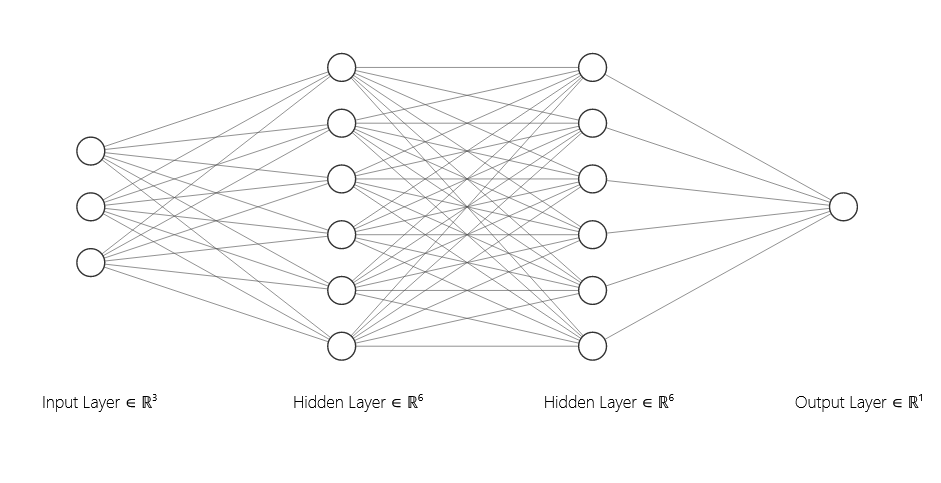
\includegraphics[width=.78\textwidth]{Theory/plots/NN.png}

\caption{A simple neural network with 3 input nodes, two hidden layers each with 6 nodes, and a output node.}
\label{fig:ML:NN}
\end{figure}

More specifically, layers in a NN include an input, an output, 
and one or multiple hidden layers.
These connections are quantified by weights $w_i$, 
where $i$ represents the index of the input node in the previous
layer. The input to a node in $n+1^{\text{th}}$ layer is given by the weighted sum of the outputs of the
nodes in the previous layer (the $n^{\text{th}}$ layer):
\[
   y^{n+1} = \sum_i^{N^n} w_i^n x_i^n + b^n,   
\addtag \]
where $N_n$ is the number of nodes,
$y^{n+1}$ is the intput to the node, $x_i^n$ is the output of the $i^{\text{th}}$ node,  
$b^n$ is the \textit{bias} which shifts the $w_i^n x_i^n$ by a certain amount.
A node then takes this input and performs a non-linear transformation using an activation function
to form its output.
There are a few frequently used activation functions, such as the sigmoid function: 
$x^{n+1} = \frac{e^{y^{n+1}}}{e^{y^{n+1}} + 1}$, or simply $\tanh(y^{n+1})$,
where the output is limited to range $[-1, 1]$;
or the rectified linear unit (ReLU), given by $x^{n+1} = max(0, y^{n+1})$, that 
has output in range $[0, 1]$.

Once the architecture of the NN is chosen, the next question is how to determine the 
weights and bias of the network.
The performance of the network for a certain task can be quantified by the \textit{loss function}.
While many different types of functions serve the purpose, one can consider a simple example that
$L(y, \hat{y}) = \frac{1}{m} \sum_{i=1}m (y_i - \hat{y_i})^2$,
where $L(y, \hat{y})$ is the loss function, $y$ is the expected output and $\hat{y}$ is
the actual output that the network gives, for $m$ test data.
To improve the performance of the NN, or equivalently minimising the loss function, 
one can `train' the NN provided with data.
The training data for the NN used in this thesis consists of pairs 
of lablled input variables and expected output, meaning the training is \textit{supervised}.
The data set used for training can be categorised into training, validation and test data sets, 
where the first two are frequently combined together for cross-validation. 
% % where a different chunk of the data is used at each training step to estimate the 
% % predictive power of a model. 

During training, the gradient of the loss function with respect to the weight and bias
is computed. The weight and bias are varied in the negative gradient direction by a small amount. 
This process is performed for multiple iterations (\textit{epochs}) until the loss function reaches its minimum.
The size of each step is control by the \textit{learning rate}.
This iterative process is known as \textit{gradient descent}.

For a large training set, the computational time for the gradient of the loss function might be very long, 
since the loss function is function of all data set. 
In this thesis, the \textit{stochastic gradient descent}~\cite{Goodfellow-et-al-2016}
method is used. Instead of computing the gradient using all data, 
the data set is divided into small \textit{batches} 
which are used to calculate an approximate gradient.

The similar problem happens when the number of connections
become large, which can happen quite easily even with a small number of nodes in each layer.
Commonly the \textit{backpropagation} algorithm is used, which 
adjust the weights and bias of one layer according to the expected output of the next layer.
For example, if the final output of the network is 0.5 while 
one expects 1, the output can be increased by boosting the weights of the connections 
to the previous layer with positive weights and to nodes with large values, and vice versa.
The weights are then updated from one layer to the layer before it (hence the term `backpropagation')
using the chain rule.

In addition, a \textit{momentum} is used in this thesis to the gradient descent 
algorithm that allows the search to build inertia in a direction in the search space and overcome 
the oscillations of noisy gradients and cross over flat spots of the search space.


The architecture of the NN (number of layers and nodes), 
learning rate, number of batches, choice of the activation functions and momentum 
are called collectively as \textit{hyperparameters}.
Unlike the weights which are learned during training, 
the hyperparameters are set before training is performed.
Depending on the data patterns to be learned or abstracted,
different values of the hyperparameters will be needed for the same ML tool.
The optimisation of the hyperparameters of the NN used in this thesis
is outlined in section~\ref{section:MVA hyper-parameters}.
